%% LoGST presentation — 3 slides
%% Compile: tectonic slides.tex
\documentclass[aspectratio=169,12pt]{beamer}
\usetheme{Madrid}
\usecolortheme{whale}
\usepackage{booktabs}
\usepackage{multirow}
\usepackage{tikz}
\usetikzlibrary{arrows.meta,positioning,fit,backgrounds,calc,shapes.geometric}
\usepackage{amsmath}
\usepackage{xcolor}
\usepackage{colortbl}

% ---- colour palette ---------------------------------------------------------
\definecolor{lo}{RGB}{30,100,180}    % local  — blue
\definecolor{gl}{RGB}{200,80,20}     % global — orange
\definecolor{sl}{RGB}{40,140,80}     % slide  — green
\definecolor{head}{RGB}{120,40,140}  % head   — purple
\definecolor{light}{RGB}{240,244,252}

\setbeamertemplate{navigation symbols}{}
\setbeamertemplate{footline}[frame number]

\newcommand{\morph}{\textsc{LoGST}}

% ---- macros for tables ------------------------------------------------------
\newcommand{\best}[1]{{\bfseries #1}}

% =============================================================================
\begin{document}

% =========================================================== SLIDE 1: ARCH ===
\begin{frame}[shrink=18]{\morph{} Architecture — Coordinate-Invariant Local-Global Spatial Transformer}

\begin{columns}[T]

%% --- Left: concept ---------------------------------------------------------
\begin{column}{0.40\textwidth}
\small
\textbf{Task:} Predict gene expression at every tissue spot from H\&E patch features.

\medskip
\textbf{Input (per slide):}
\begin{itemize}
  \item $\mathbf{F}\in\mathbb{R}^{N\times1536}$ — frozen UNI+CONCH patch embeddings
  \item $\mathbf{C}\in\mathbb{R}^{N\times2}$ — spot pixel coordinates
\end{itemize}

\medskip
\textbf{Output:}
$\hat{\mathbf{E}}\in\mathbb{R}^{N\times50}$ — predicted log-normalised expression

\medskip
\textbf{Coordinate invariance:}\\
Coordinates enter \emph{only} via pairwise distances (RBF-encoded).\\
$\Rightarrow$ invariant to translation, rotation \& reflection.

\medskip
\textbf{Single forward pass} — 4.88\,M params
\end{column}

%% --- Right: architecture diagram -------------------------------------------
\begin{column}{0.58\textwidth}
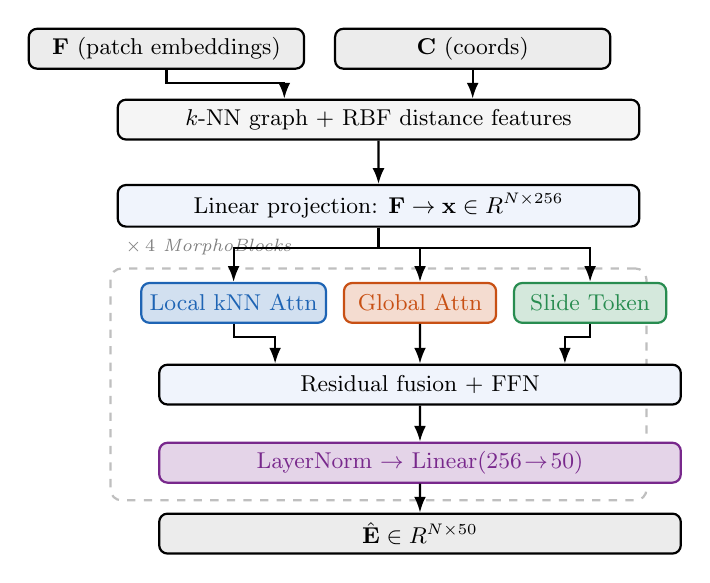
\begin{tikzpicture}[
  every node/.style={font=\small},
  box/.style={rounded corners=3pt, draw, thick, minimum width=3.8cm,
              minimum height=0.55cm, align=center},
  arr/.style={-{Latex[length=2mm]}, thick},
  scale=0.92, transform shape
]

%% Input
\node[box, fill=gray!15] (inp) {$\mathbf{F}$ (patch embeddings)};
\node[box, fill=gray!15, right=0.4cm of inp] (crd) {$\mathbf{C}$ (coords)};

%% kNN + RBF
\node[box, fill=gray!8, below=0.4cm of crd, xshift=-1.3cm,
      minimum width=7.2cm]
  (rbf) {$k$-NN graph $+$ RBF distance features};

%% Linear projection
\node[box, fill=light, below=0.6cm of rbf, minimum width=7.2cm] (proj)
  {Linear projection: $\mathbf{F}\to\mathbf{x}\in\mathbb{R}^{N\times 256}$};

%% Block (repeated)
\node[draw=gray!50, rounded corners=4pt, dashed, thick,
      below=0.55cm of proj, minimum width=7.4cm, minimum height=3.2cm]
  (blk) {};
\node[above right=0.05cm and 0.1cm of blk.north west, font=\scriptsize\itshape, gray]
  {$\times\,4$ MorphoBlocks};

%% Three streams inside block
\node[box, fill=lo!20, draw=lo, below=0.75cm of proj, xshift=-2.0cm,
      minimum width=2.1cm] (loc)
  {\textcolor{lo}{Local kNN Attn}};
\node[box, fill=gl!20, draw=gl, right=0.22cm of loc,
      minimum width=2.1cm] (glo)
  {\textcolor{gl}{Global Attn}};
\node[box, fill=sl!20, draw=sl, right=0.22cm of glo,
      minimum width=2.1cm] (slt)
  {\textcolor{sl}{Slide Token}};

%% Fusion + FFN
\node[box, fill=light, below=0.55cm of glo, minimum width=7.2cm] (fuse)
  {Residual fusion $+$ FFN};

%% Head
\node[box, fill=head!20, draw=head, below=0.5cm of fuse, minimum width=7.2cm] (head)
  {\textcolor{head}{LayerNorm $\to$ Linear$(256\!\to\!50)$}};

%% Output
\node[box, fill=gray!15, below=0.4cm of head, minimum width=7.2cm] (out)
  {$\hat{\mathbf{E}}\in\mathbb{R}^{N\times50}$};

%% Arrows
\draw[arr] (inp.south) -- ++(0,-0.18) -| ([xshift=-1.3cm]rbf.north);
\draw[arr] (crd.south) -- ++(0,-0.18) -| ([xshift=+1.3cm]rbf.north);
\draw[arr] (rbf) -- (proj);
\draw[arr] (proj.south) -- ++(0,-0.28) -| (loc.north);
\draw[arr] (proj.south) -- ++(0,-0.28) -| (glo.north);
\draw[arr] (proj.south) -- ++(0,-0.28) -| (slt.north);
\draw[arr] (loc.south) -- ++(0,-0.18) -| ([xshift=-2.0cm]fuse.north);
\draw[arr] (glo.south) -- (fuse.north);
\draw[arr] (slt.south) -- ++(0,-0.18) -| ([xshift=+2.0cm]fuse.north);
\draw[arr] (fuse) -- (head);
\draw[arr] (head) -- (out);

\end{tikzpicture}
\end{column}
\end{columns}

\end{frame}


% =========================================================== SLIDE 2: RESULTS (T1, T2) ===
\begin{frame}{Results — Intra-Cohort (Table 1) \& Cross-Organ LOOO (Table 2)}

\begin{columns}[T]

%% ---- Table 1 ---------------------------------------------------------------
\begin{column}{0.52\textwidth}
\centering
{\small\textbf{Table 1: Intra-cohort PCC per organ (HEST-1k)}}\\[2pt]
{\scriptsize All methods: frozen UNI+CONCH, 50 genes, 3 seeds}

\medskip
\resizebox{\columnwidth}{!}{%
\begin{tabular}{l ccc cc c}
\toprule
Cohort & ST-Net & Hist2ST & HyperST & BLEEP & STEM & \morph{} \\
\midrule
IDC (Breast)      & 0.551 & 0.309 & 0.567 & 0.519 & 0.439 & \best{0.581} \\
COAD (Colorectal) & 0.242 & 0.295 & 0.285 & 0.314 & 0.177 & \best{0.318} \\
CCRCC (Kidney)    & 0.163 & 0.184 & \best{0.256} & 0.175 & 0.123 & 0.252 \\
LUNG              & 0.518 & 0.470 & 0.587 & 0.562 & 0.423 & \best{0.589} \\
PAAD (Pancreas)   & 0.359 & 0.247 & 0.404 & 0.419 & 0.233 & \best{0.437} \\
PRAD (Prostate)   & 0.294 & 0.333 & 0.384 & 0.348 & 0.207 & \best{0.410} \\
SKCM (Skin)       & 0.665 & 0.522 & 0.653 & 0.645 & 0.491 & \best{0.707} \\
\midrule
\textbf{Average}  & 0.399 & 0.337 & 0.448 & 0.426 & 0.299 & \best{0.470} \\
\bottomrule
\end{tabular}%
}

\smallskip
{\footnotesize \textcolor{lo}{\textbf{+6.6\%}} relative PCC gain over best baseline (HyperST)}
\end{column}

\hfill
%% ---- Table 2 ---------------------------------------------------------------
\begin{column}{0.46\textwidth}
\centering
{\small\textbf{Table 2: Cross-organ LOOO PCC per organ}}\\[2pt]
{\scriptsize Trained on 6 organs, tested on held-out organ}

\medskip
\resizebox{\columnwidth}{!}{%
\begin{tabular}{l ccc c c}
\toprule
Cohort & ST-Net & Hist2ST & HyperST & BLEEP & \morph{} \\
\midrule
IDC (Breast)      & 0.198 & 0.458 & 0.465 & \best{0.529} & 0.520 \\
COAD (Colorectal) & 0.420 & 0.670 & 0.669 & 0.662 & \best{0.729} \\
CCRCC (Kidney)    & 0.068 & 0.055 & 0.106 & 0.095 & \best{0.109} \\
LUNG              & 0.493 & 0.378 & 0.657 & 0.624 & \best{0.675} \\
PAAD (Pancreas)   & 0.459 & 0.399 & 0.463 & 0.537 & \best{0.548} \\
PRAD (Prostate)   & 0.079 & 0.098 & 0.114 & 0.118 & \best{0.118} \\
SKCM (Skin)       & 0.520 & 0.736 & 0.725 & \best{0.748} & 0.728 \\
\midrule
\textbf{Average}  & 0.319 & 0.399 & 0.457 & 0.473 & \best{0.490} \\
\bottomrule
\end{tabular}%
}

\smallskip
{\footnotesize \morph{} leads on 5/7 organs under organ-shift transfer}
\end{column}

\end{columns}

\end{frame}


% =========================================================== SLIDE 3: ABLATION + INVARIANCE ===
\begin{frame}[shrink=12]{Results — Ablation (Table 7) \& Coordinate Invariance (Table 8)}

\begin{columns}[T]

%% ---- Table 7 ---------------------------------------------------------------
\begin{column}{0.54\textwidth}
\centering
{\small\textbf{Table 7: Factorial Context Ablation (Intra-cohort)}}\\[2pt]
{\scriptsize L=Local attention,\; G=Global attention,\; S=Slide token}

\medskip
\resizebox{\columnwidth}{!}{%
\begin{tabular}{l ccc cc c}
\toprule
Config & L & G & S & SKCM & LUNG & Avg \\
\midrule
C000 (MLP only) & & & & 0.639 & 0.577 & 0.608 \\
C001 & & & $\bullet$ & 0.633 & 0.578 & 0.605 \\
C010 & & $\bullet$ & & 0.641 & 0.577 & 0.609 \\
C011 & & $\bullet$ & $\bullet$ & 0.639 & 0.583 & 0.611 \\
C100 & $\bullet$ & & & 0.693 & 0.587 & 0.640 \\
C101 & $\bullet$ & & $\bullet$ & 0.695 & 0.585 & 0.640 \\
C110 & $\bullet$ & $\bullet$ & & 0.693 & 0.584 & 0.638 \\
\rowcolor{lo!12}
C111 (\morph{}) & $\bullet$ & $\bullet$ & $\bullet$ & \best{0.696} & \best{0.589} & \best{0.643} \\
\bottomrule
\end{tabular}%
}

\smallskip
{\footnotesize
  Local attention ($+$0.032 avg) is the dominant single contributor.\\
  All three components together achieve the best performance.
}
\end{column}

\hfill
%% ---- Table 8 ---------------------------------------------------------------
\begin{column}{0.43\textwidth}
\centering
{\small\textbf{Table 8: Numerical Coordinate-Invariance Check}}\\[2pt]
{\scriptsize Randomly initialised model, 257-spot synthetic slide.\\
Max.\ absolute output difference after coordinate transformation.}

\medskip
\begin{tabular}{l r}
\toprule
Transformation & Max.\ $|\Delta|$ \\
\midrule
Translation      & $5.97\!\times\!10^{-5}$ \\
Rotation         & $1.97\!\times\!10^{-5}$ \\
Reflection       & $0$ \\
Spot permutation & $5.96\!\times\!10^{-7}$ \\
\bottomrule
\end{tabular}

\bigskip
{\footnotesize
Differences are numerical noise ($<\!10^{-4}$), confirming predictions are invariant to how the tissue slide is oriented or positioned.

\medskip
\textbf{Why it matters:} Two labs imaging the same tissue with different coordinate origins or rotated stage orientations get \emph{identical} predictions.
}
\end{column}

\end{columns}

\end{frame}

\end{document}
